\section{Resultados}
\label{sec:resultados}

\subsection{Verificación de corrección}
En todas las instancias del benchmark, las tres colas produjeron las mismas distancias y el certificado de optimalidad se cumplió. La comparación con NetworkX no detectó discrepancias y el certificado de Bellman recorrió todas las aristas y caminos sin violaciones. En la consulta OSM, las tres colas devolvieron la misma ruta y el mismo costo base de $387.197$ s. La igualdad de distancias es la condición mínima para que la comparación de tiempos tenga sentido: si las colas resolvieran problemas distintos, el tiempo no sería comparable.

\subsection{Benchmark sintético}
Las Tablas~\ref{tab:benchmark_sparse} y~\ref{tab:benchmark_dense} presentan la mediana y el IQR de 45 muestras por celda (tres instancias $\times$ 15 repeticiones). La Figura~\ref{fig:benchmark_canonico} muestra las curvas en escala logarítmica; las barras de error corresponden al IQR.

\begin{table}[H]
\centering
\fontsize{9}{10.5}\selectfont
\renewcommand{\arraystretch}{1.12}
\setlength{\tabcolsep}{4pt}
\caption{Dijkstra con tres colas, perfil disperso: mediana e IQR en $\mu$s.}
\label{tab:benchmark_sparse}
\begin{tabular}{@{}rrccc l@{}}
\toprule
$|V|$ & $|E|$ & \makecell{Binary\\Heap} & \makecell{4-ary\\Heap} & \makecell{Fibonacci\\Heap} & Mejor \\
\midrule
100 & 400 & \makecell{1648.4\\{\scriptsize[1377.9, 1979.3]}} & \makecell{1673.3\\{\scriptsize[1393.8, 2186.5]}} & \makecell{2574.3\\{\scriptsize[2371.2, 2870.8]}} & Binary \\
500 & 2000 & \makecell{19232.5\\{\scriptsize[14655.3, 24254.5]}} & \makecell{14531.3\\{\scriptsize[11524.1, 18064.2]}} & \makecell{30497.4\\{\scriptsize[20429.6, 38086.3]}} & 4-ary \\
1000 & 4000 & \makecell{43378.1\\{\scriptsize[37780.5, 54962.6]}} & \makecell{41803.4\\{\scriptsize[33976.3, 53954.7]}} & \makecell{58348.7\\{\scriptsize[47548.7, 65855.4]}} & 4-ary \\
2500 & 10000 & \makecell{105786.6\\{\scriptsize[96970.5, 121834.1]}} & \makecell{106339.6\\{\scriptsize[94379.9, 122938.1]}} & \makecell{138649.1\\{\scriptsize[121508.9, 170908.3]}} & Binary \\
5000 & 20000 & \makecell{254749.2\\{\scriptsize[219442.6, 316895.6]}} & \makecell{212803.0\\{\scriptsize[199918.1, 232243.5]}} & \makecell{285718.4\\{\scriptsize[261162.8, 315459.6]}} & 4-ary \\
\bottomrule
\end{tabular}
\par\vspace{0.1cm}
\raggedright\fontsize{8.5}{10.5}\selectfont\textit{Nota.} Cada celda muestra la mediana y, entre corchetes, el IQR.
\end{table}

\begin{table}[H]
\centering
\fontsize{9}{10.5}\selectfont
\renewcommand{\arraystretch}{1.12}
\setlength{\tabcolsep}{4pt}
\caption{Dijkstra con tres colas, perfil denso: mediana e IQR en $\mu$s.}
\label{tab:benchmark_dense}
\begin{tabular}{@{}rrccc l@{}}
\toprule
$|V|$ & $|E|$ & \makecell{Binary\\Heap} & \makecell{4-ary\\Heap} & \makecell{Fibonacci\\Heap} & Mejor \\
\midrule
50 & 196 & \makecell{892.0\\{\scriptsize[821.0, 1074.6]}} & \makecell{872.9\\{\scriptsize[783.2, 994.0]}} & \makecell{1284.4\\{\scriptsize[1132.8, 1411.3]}} & 4-ary \\
100 & 792 & \makecell{2287.0\\{\scriptsize[2057.4, 3227.4]}} & \makecell{2182.2\\{\scriptsize[1894.3, 2405.6]}} & \makecell{3142.8\\{\scriptsize[2655.2, 3976.6]}} & 4-ary \\
200 & 3184 & \makecell{5138.6\\{\scriptsize[4040.9, 6430.3]}} & \makecell{4852.3\\{\scriptsize[3881.0, 6065.4]}} & \makecell{7169.3\\{\scriptsize[5476.0, 8327.4]}} & 4-ary \\
400 & 12768 & \makecell{16408.9\\{\scriptsize[13090.2, 18599.3]}} & \makecell{15487.6\\{\scriptsize[12208.9, 19884.7]}} & \makecell{17183.7\\{\scriptsize[15487.0, 21265.9]}} & 4-ary \\
800 & 51136 & \makecell{57923.5\\{\scriptsize[50208.7, 62974.9]}} & \makecell{58345.2\\{\scriptsize[50691.3, 68398.6]}} & \makecell{74614.7\\{\scriptsize[60800.1, 89075.6]}} & Binary \\
\bottomrule
\end{tabular}
\par\vspace{0.1cm}
\raggedright\fontsize{8.5}{10.5}\selectfont\textit{Nota.} Cada celda muestra la mediana y, entre corchetes, el IQR.
\end{table}


\begin{figure}[H]
    \centering
    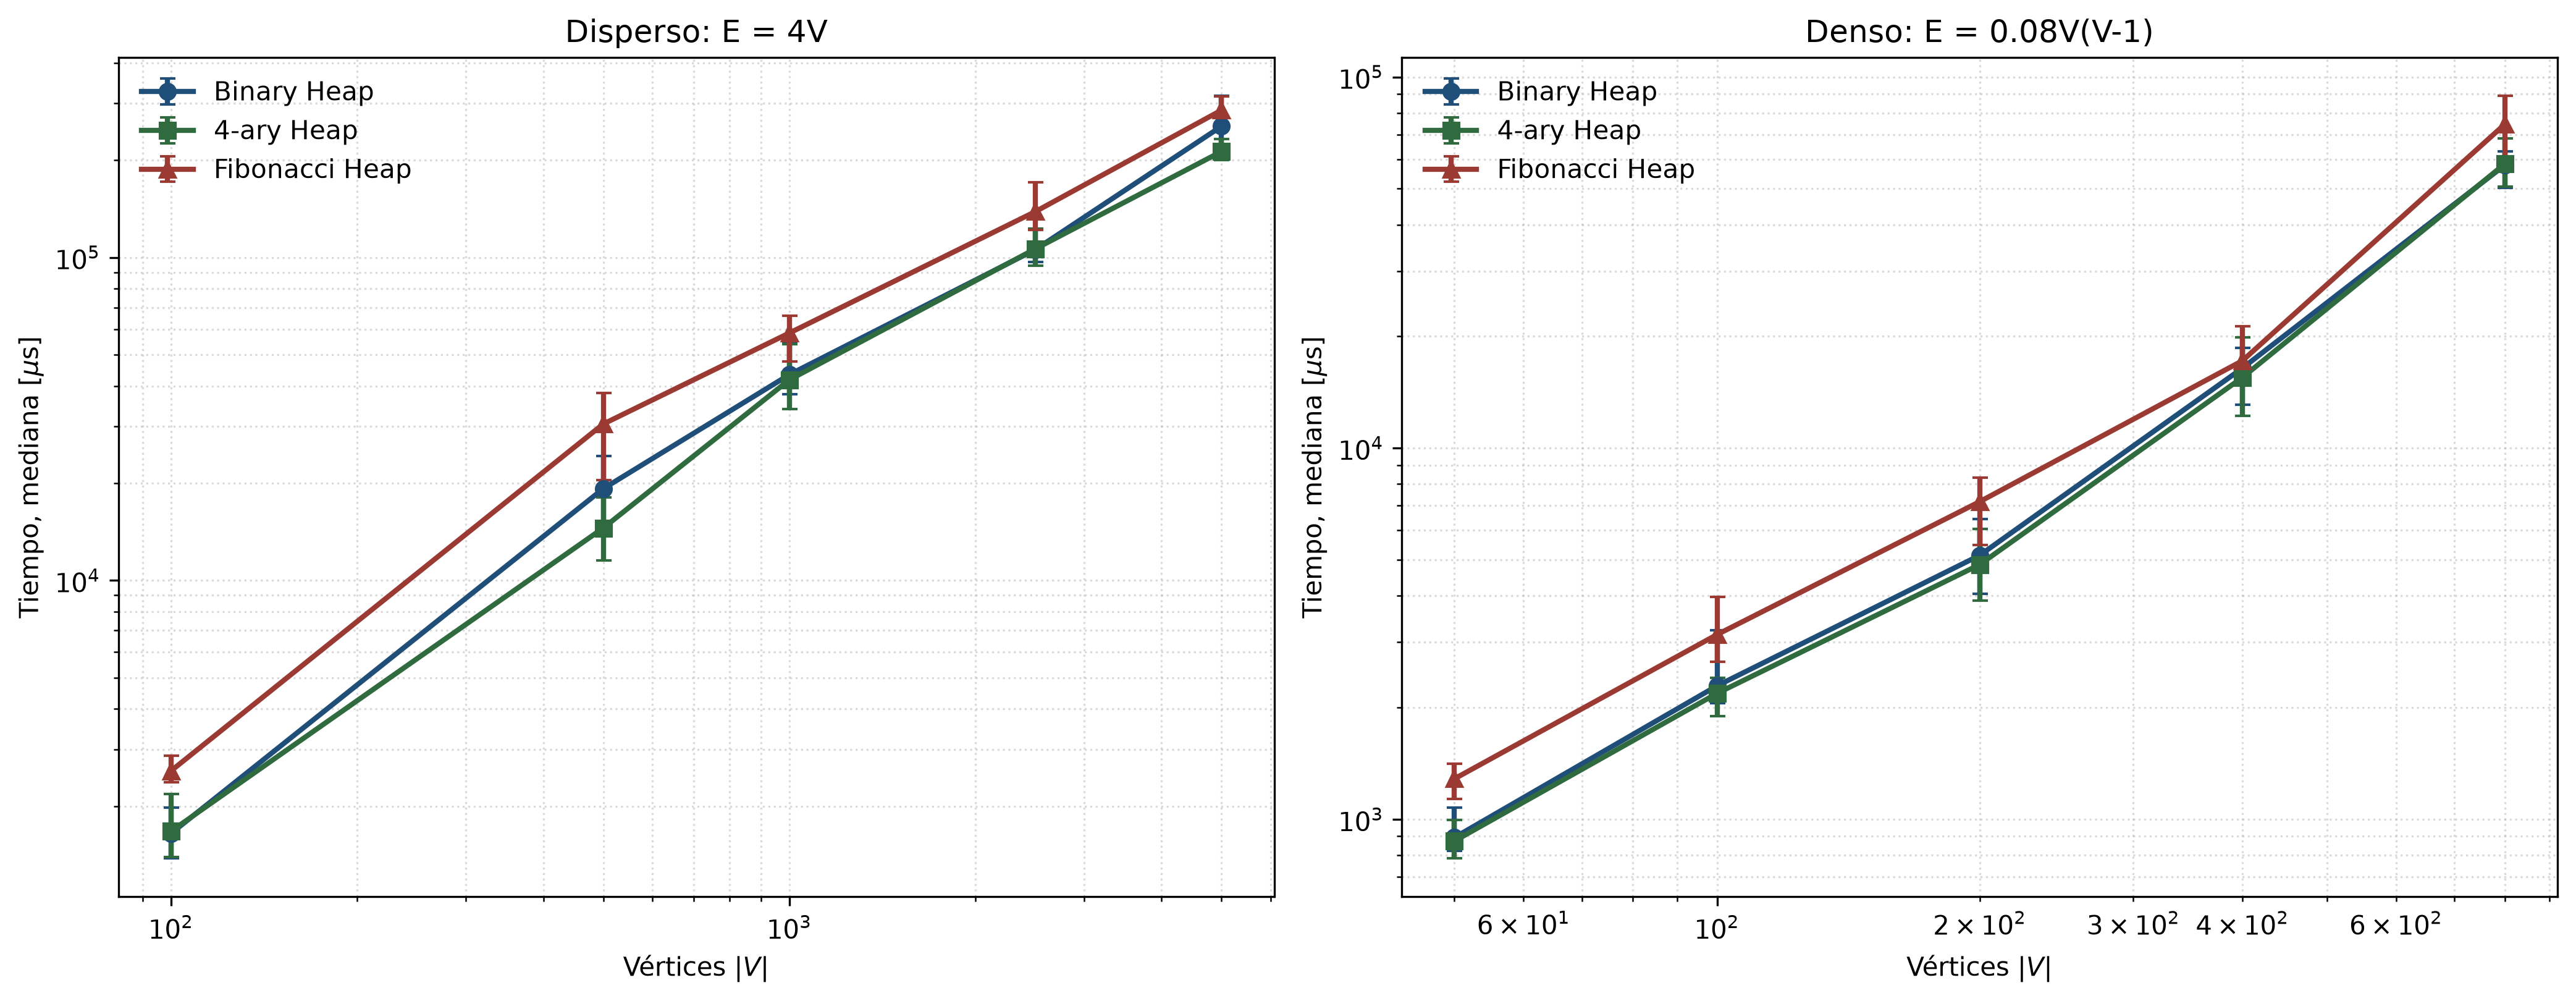
\includegraphics[width=\textwidth]{figuras/benchmark_canonico.png}
    \caption{Tiempo mediano de Dijkstra con las tres colas. Izquierda: perfil disperso ($|E|=4|V|$). Derecha: perfil denso ($|E|=0.08|V|(|V|-1)$). Las barras verticales representan el IQR.}
    \label{fig:benchmark_canonico}
\end{figure}

\paragraph{Perfil disperso.} El heap 4-ario obtuvo la menor mediana en 3 de 5 escalas (500, 1000 y 5000), y el binario en 2 (100 y 2500). La razón mediana 4-ario/binario fue $0.964$; es decir, el 4-ario fue un 3.6\,\% más rápido en la mediana de las escalas, pero la diferencia cambia de signo: fue 24.4\,\% más rápido en $|V|=500$, 3.6\,\% en $|V|=1000$, 16.5\,\% en $|V|=5000$, y 1.5\,\% y 0.5\,\% más lento en $|V|=100$ y $|V|=2500$. Los IQR de ambas colas se solapan en las cinco escalas, por lo que la ventaja no es concluyente en ninguna escala individual.

\paragraph{Perfil denso.} El 4-ario ganó 4 de 5 escalas (50, 100, 200 y 400) y el binario ganó en $|V|=800$. La razón mediana fue $0.954$ (4.6\,\% más rápido), con ventajas de 2.1\,\%, 4.6\,\%, 5.6\,\% y 5.6\,\% en las cuatro escalas ganadas, y una desventaja de 0.7\,\% en $|V|=800$. Los IQR se solapan en las cinco escalas. La densidad no produjo un cambio cualitativo: el 4-ario conserva una ventaja pequeña y variable, no una superioridad sistemática.

\paragraph{Fibonacci heap.} El Fibonacci heap no obtuvo la menor mediana en ninguna de las 10 escalas. Fue entre 1.05 y 1.59 veces más lento que el binario; en el perfil disperso, el rango fue 1.12--1.59, y en el denso, 1.05--1.44. Los IQR de Fibonacci y binario se solapan en 8 de 10 escalas; las dos excepciones son $|V|=100$ disperso y $|V|=50$ denso, donde el Fibonacci fue claramente más lento. La dirección del resultado es consistente: la cota asintótica no se tradujo en tiempo de pared.

\begin{table}[H]
\centering
\fontsize{8.5}{10.5}\selectfont
\renewcommand{\arraystretch}{1.15}
\setlength{\tabcolsep}{4pt}
\caption{Síntesis por perfil y consulta: conteo de menores medianas observadas, sin declarar diferencias concluyentes donde se solapan los IQR.}
\label{tab:sintesis_colas}
\begin{tabular}{@{}lrrrrr@{}}
\toprule
\textbf{Perfil} & \textbf{4-ary/Binary} & \textbf{Fibonacci/Binary} & \makecell{Menor mediana\\4-ary} & \makecell{Menor mediana\\Binary} & \textbf{IQR solap.} \\
\midrule
Disperso ($|E|=4|V|$) & 0.964 & 1.345 & 3 de 5 & 2 de 5 & 5 de 5 \\
Denso ($|E|=0.08|V|(|V|-1)$) & 0.954 & 1.374 & 4 de 5 & 1 de 5 & 5 de 5 \\
\midrule
Total sintético & 0.959 & 1.360 & 7 de 10 & 3 de 10 & 10 de 10 \\
Consulta OSM & 1.269 & 1.666 & 0 & 1 & 1 de 1 \\
\bottomrule
\end{tabular}
\par\vspace{0.1cm}
\raggedright\fontsize{8}{10}\selectfont\textit{Nota.} Razón 4-ary/Binary menor que 1: menor mediana del 4-ario. IQR solap. compara 4-ary frente a Binary; el solapamiento impide afirmar superioridad inequívoca. Fibonacci no obtuvo la menor mediana en ninguna escala sintética.
\end{table}


\subsection{Operaciones elementales}
La Figura~\ref{fig:operaciones} descompone las operaciones del perfil disperso. En $|V|=5000$, las tres colas realizaron 5000 inserciones, 5000 extracciones y 6695 \texttt{decrease\_key} efectivos sobre 10415 intentos de relajación. Los intentos que no mejoran la distancia no invocan \texttt{decrease\_key}; por eso el número de decrementos es menor que $|E|$. En el perfil denso con $|V|=800$, hubo 2976 decrementos sobre 25527 intentos, es decir, solo el 11.7\,\%.

\begin{figure}[H]
    \centering
    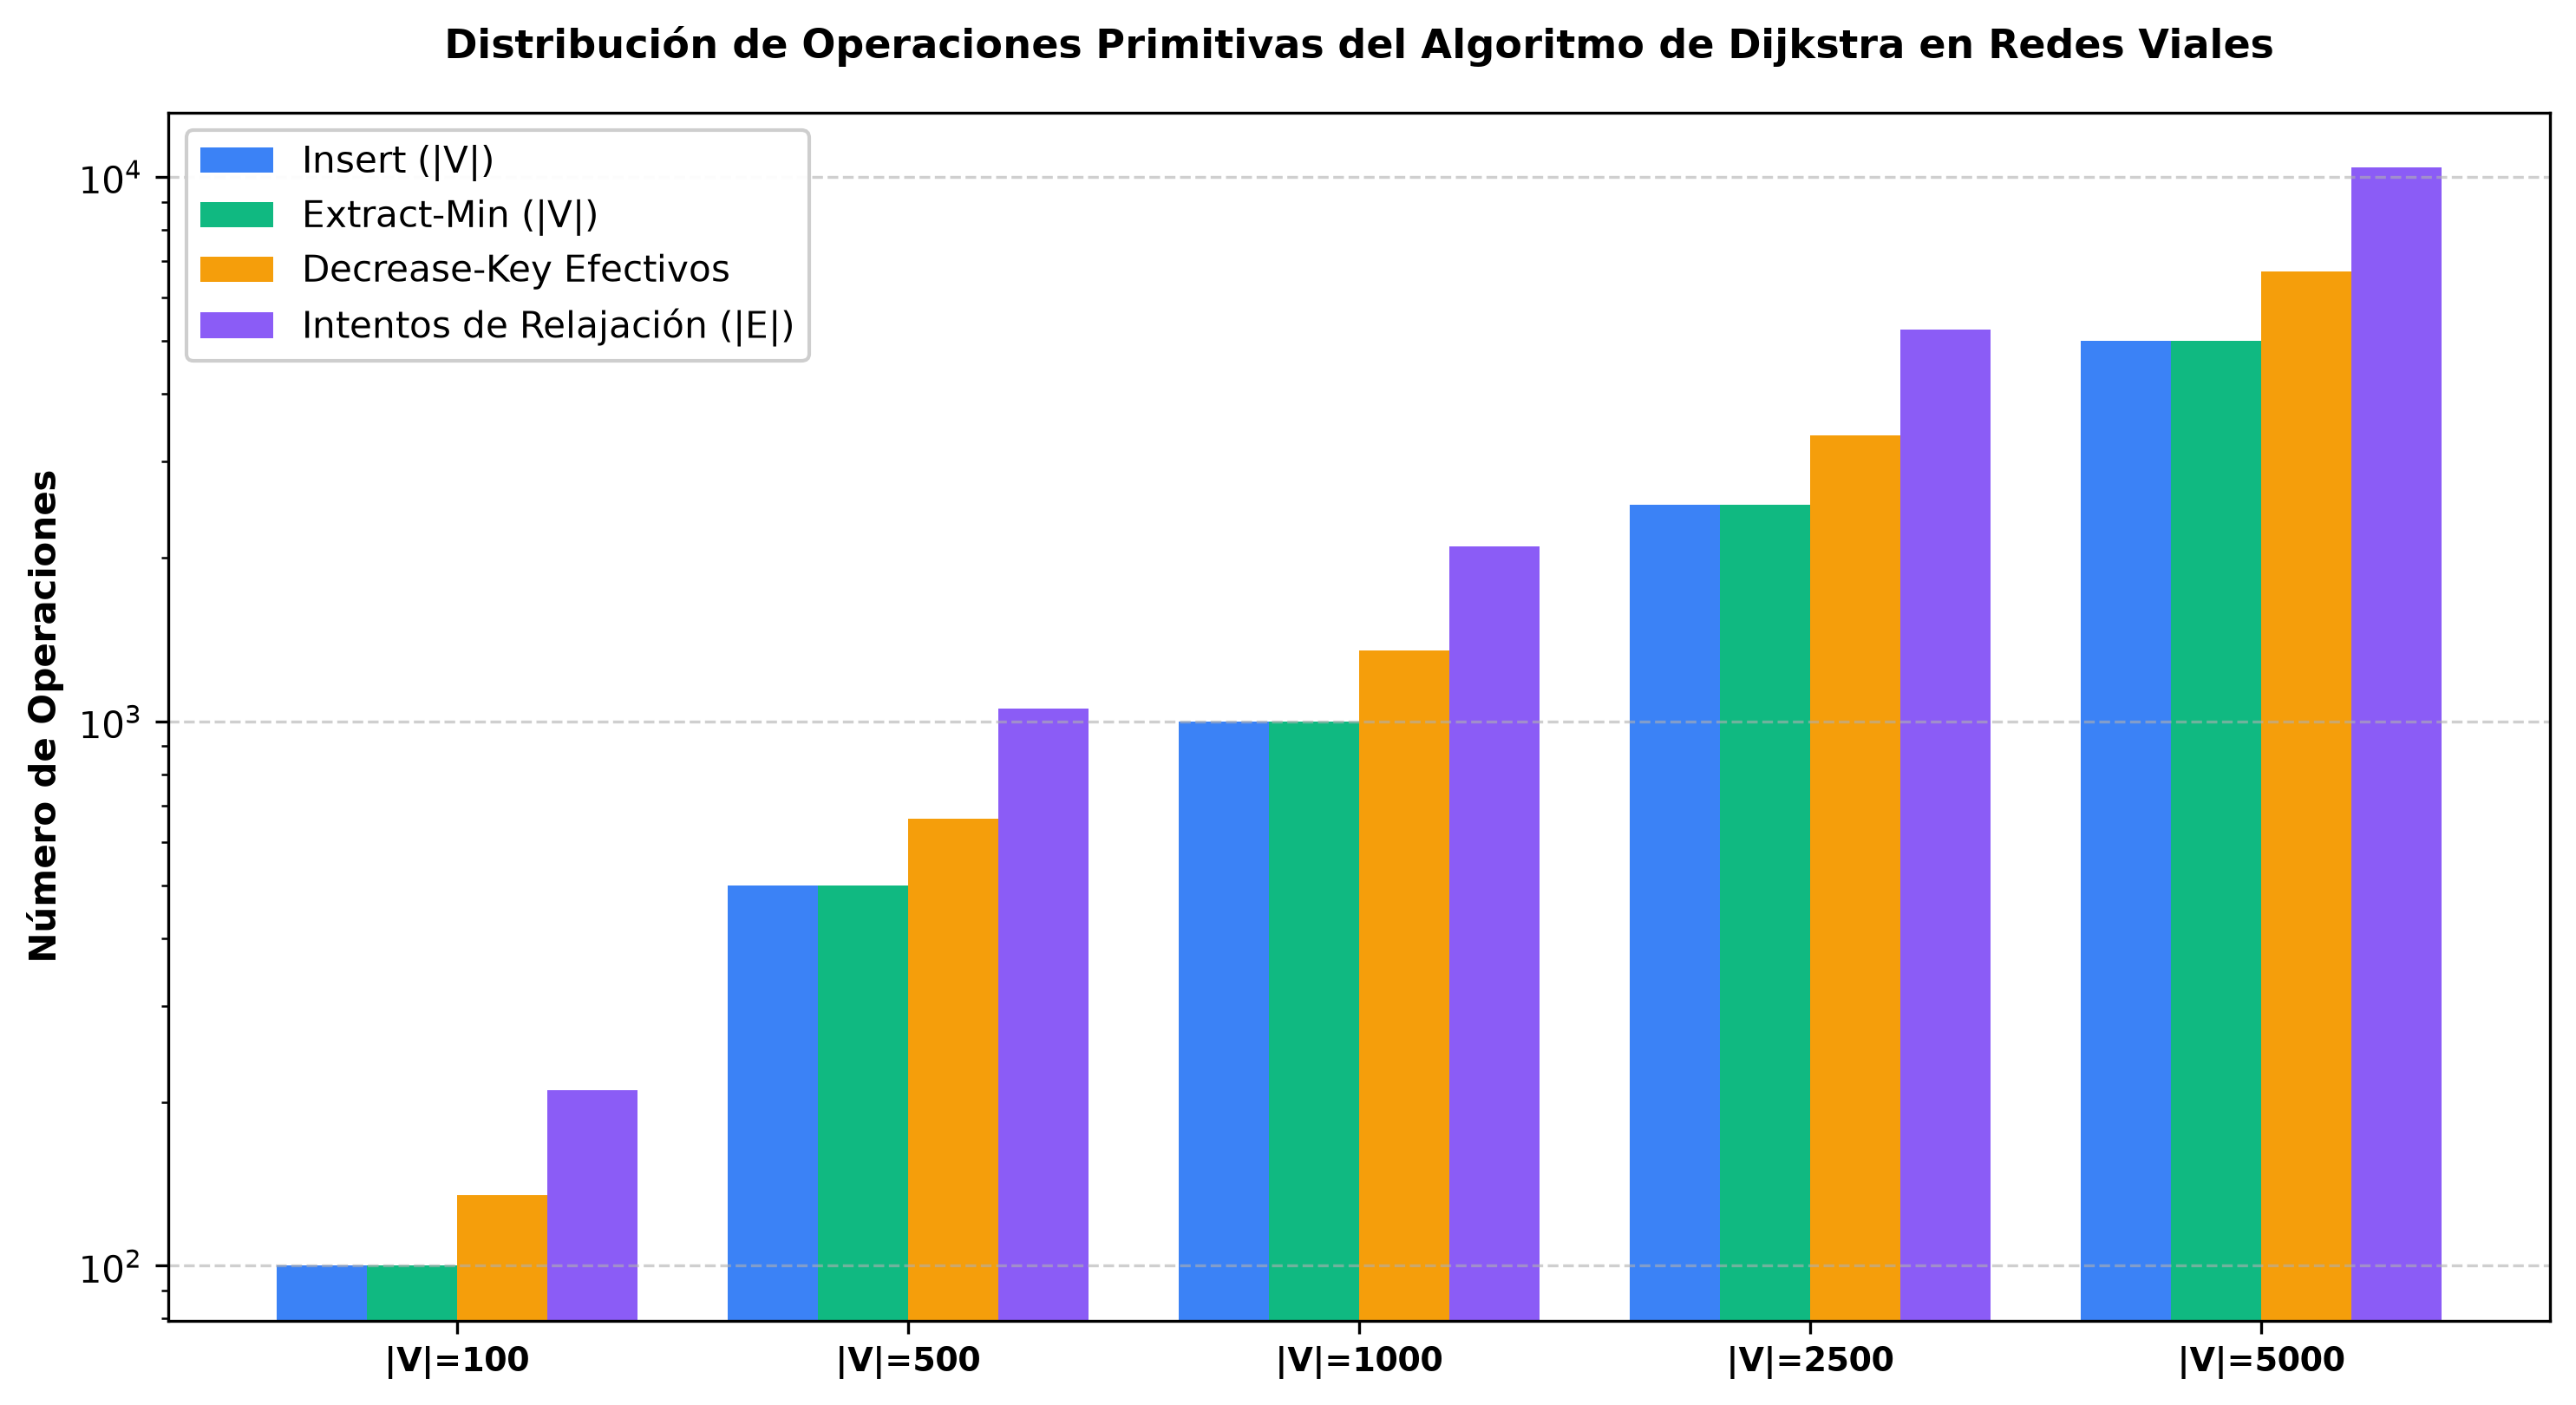
\includegraphics[width=0.92\textwidth]{figuras/operaciones_canonicas.png}
    \caption{Operaciones primitivas de Dijkstra en el perfil disperso. Las barras agrupan inserciones, extracciones, \texttt{decrease\_key} efectivos e intentos de relajación.}
    \label{fig:operaciones}
\end{figure}

El conteo de comparaciones explica solo una parte del tiempo. En $|V|=5000$ disperso, el Fibonacci heap realizó 101303 comparaciones frente a 125776 del binario (19.5\,\% menos), pero fue 12.2\,\% más lento. En $|V|=800$ denso, hizo 19848 comparaciones frente a 21280 (6.7\,\% menos) y fue 28.8\,\% más lento. La diferencia restante proviene de la manipulación de punteros, la asignación de nodos, los cortes en cascada y la consolidación, costos que no aparecen en el conteo de comparaciones. Esta observación es consistente con la literatura sobre localidad de memoria \parencite{lamarca1996cache}.

\subsection{Caso aplicado: consulta OSM en Cusco}
La red aplicada tiene 891 vértices y 2139 aristas dirigidas. La consulta seleccionada por la regla determinista va del vértice \texttt{30972889} al \texttt{5996728243}; la ruta óptima tiene 17 vértices, 2810.6 m y un costo base de 387.197 s. La Figura~\ref{fig:ruta_osm} muestra la red, la ruta y los extremos.

\begin{figure}[H]
    \centering
    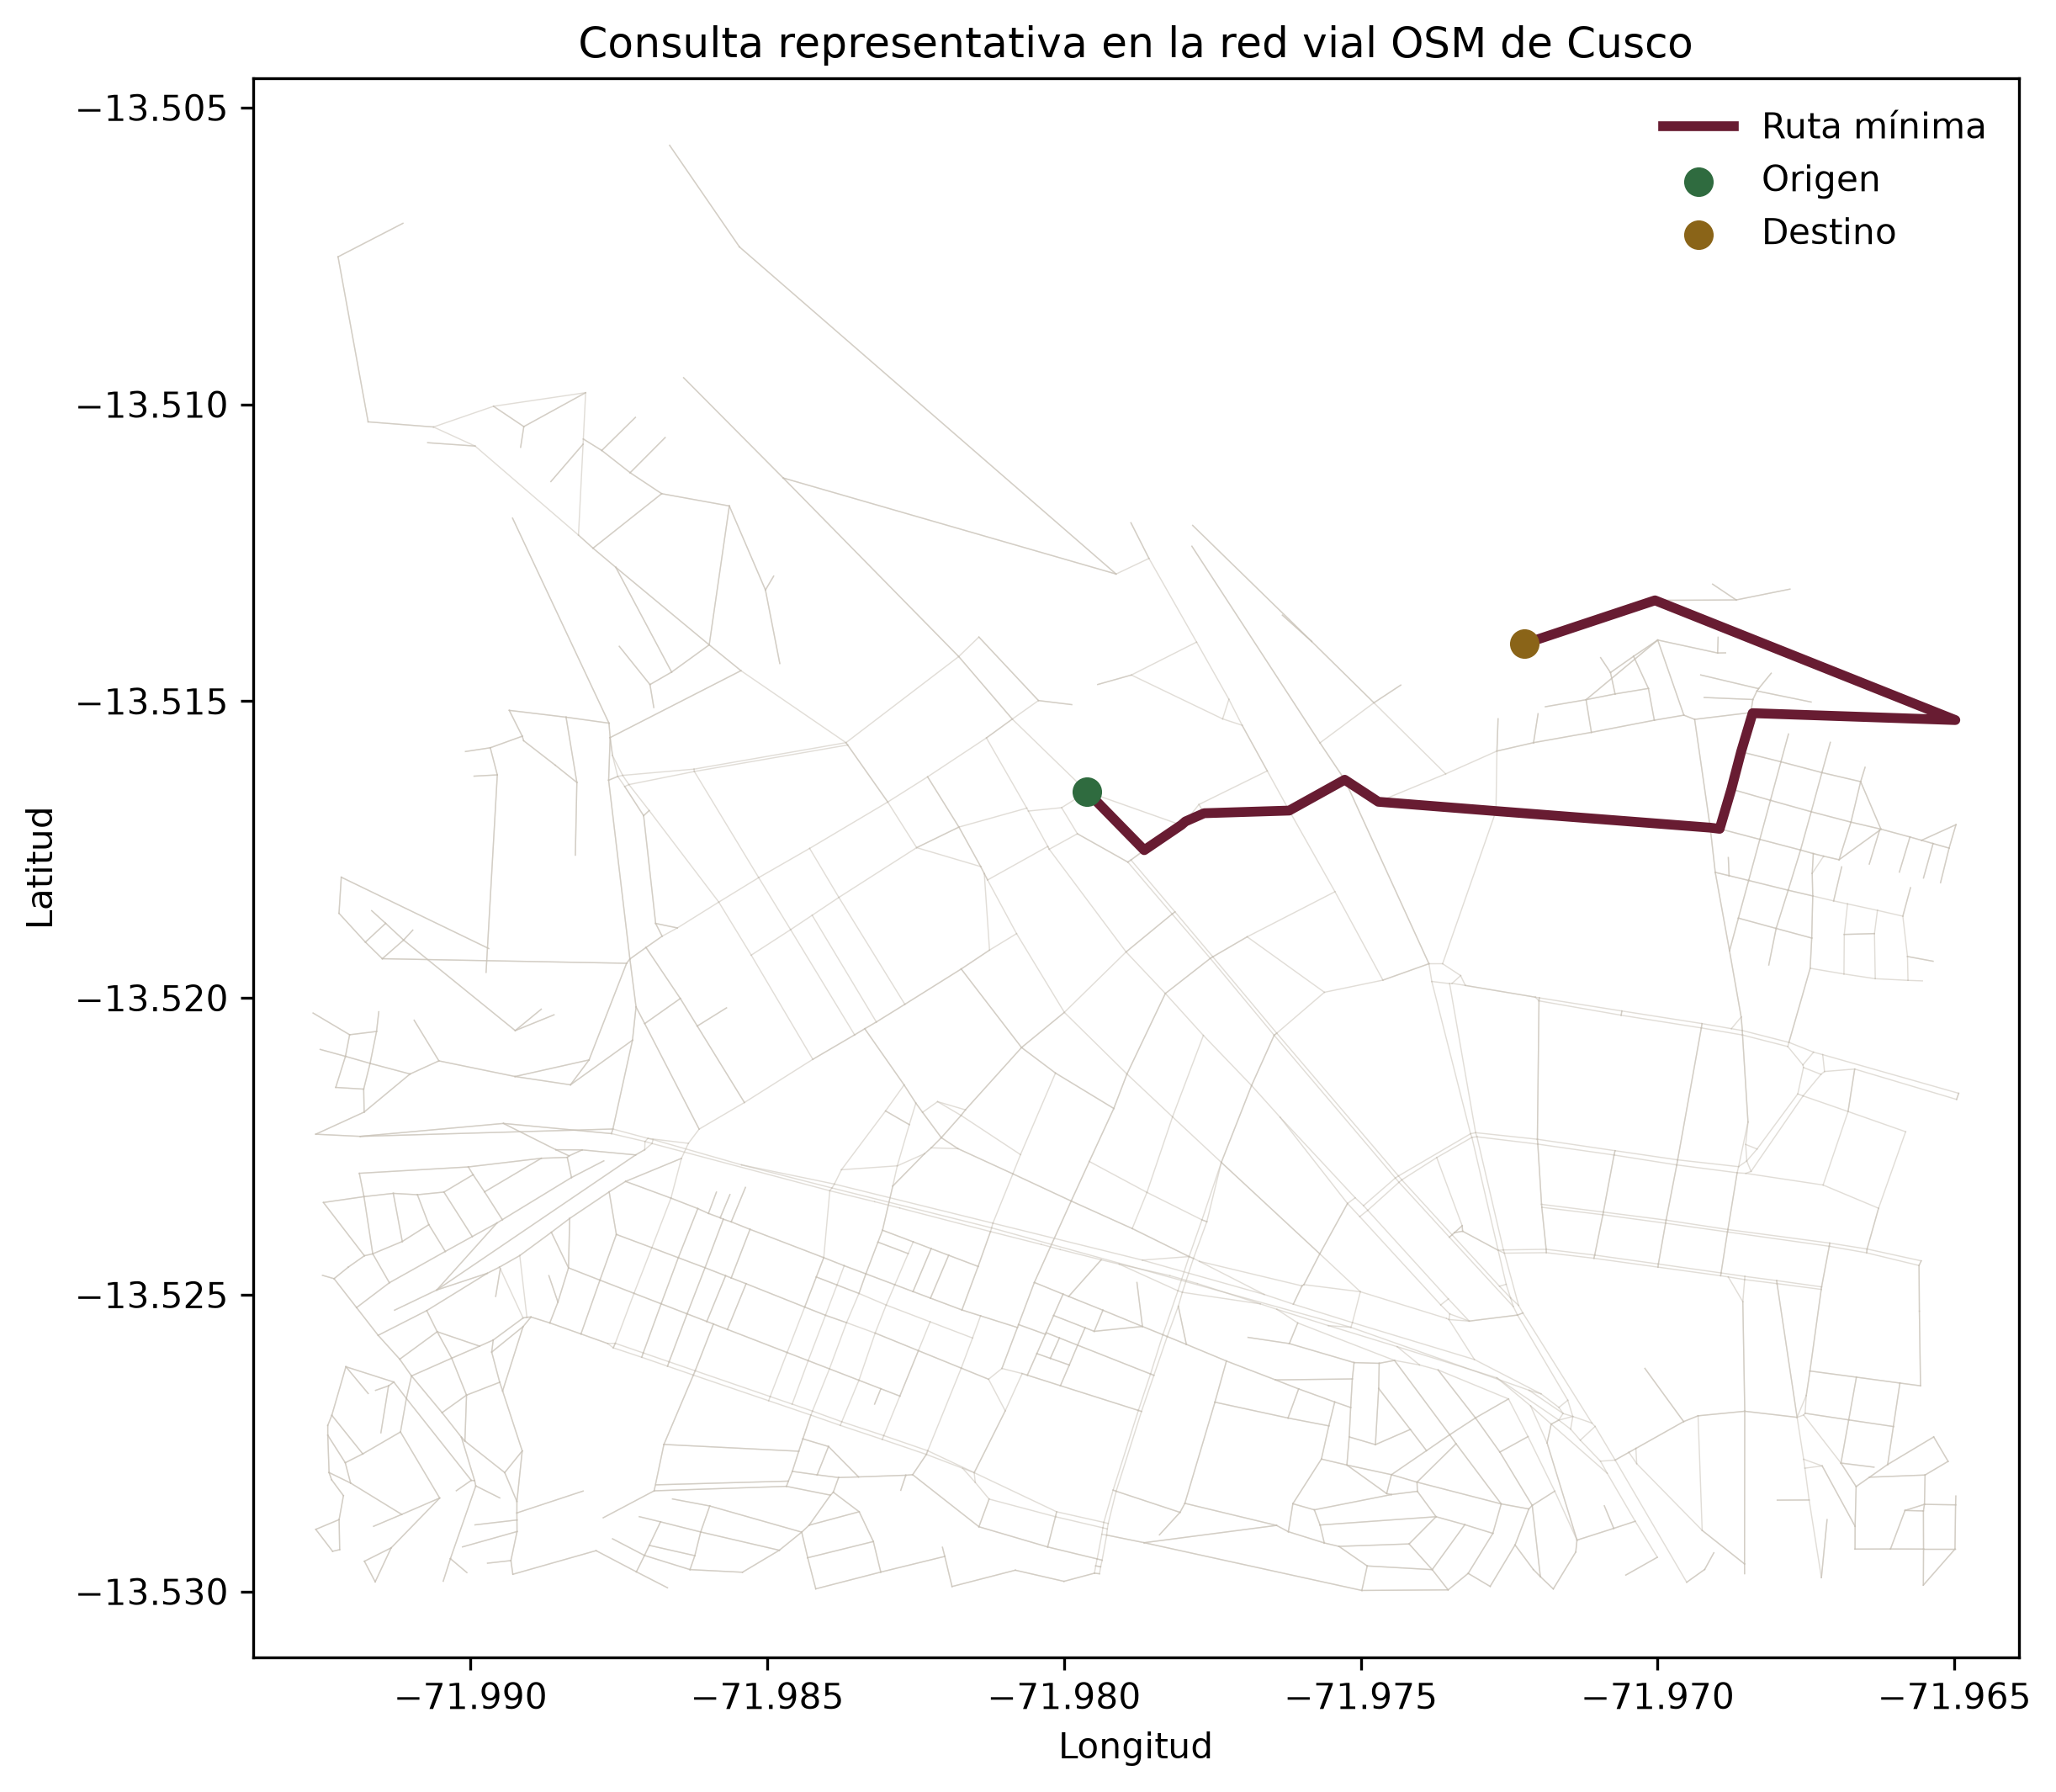
\includegraphics[width=0.86\textwidth]{figuras/ruta_osm_cusco.png}
    \caption{Ruta mínima sobre la red vial OSM de Cusco. La línea resalta el camino óptimo; los marcadores indican origen y destino.}
    \label{fig:ruta_osm}
\end{figure}

La Tabla~\ref{tab:benchmark_osm} reporta los tiempos de la consulta. El heap binario obtuvo la menor mediana (15.65 ms), seguido del 4-ario (19.87 ms, +26.9\,\%) y del Fibonacci (26.09 ms, +66.7\,\%). El IQR del binario [13.07, 19.55] se solapa con el del 4-ario [17.33, 22.68], de modo que la ventaja del binario frente al 4-ario es sugerente pero no concluyente; el IQR del Fibonacci [24.03, 27.34] no se solapa con el del binario, y su desventaja sí es clara en esta consulta.

\begin{table}[H]
\centering
\caption{Caso OSM: tiempo de Dijkstra por cola, mediana e IQR.}
\label{tab:benchmark_osm}
\begin{tabular}{lrrr}
\toprule
Cola & Mediana ($\mu$s) & Q1 ($\mu$s) & Q3 ($\mu$s) \\
\midrule
\textbf{Binary Heap} & 15655.0 & 13065.6 & 19550.7 \\
4-ary Heap & 19872.2 & 17335.0 & 22675.6 \\
Fibonacci Heap & 26088.7 & 24033.9 & 27343.9 \\
\bottomrule
\end{tabular}
\end{table}

\begin{table}[H]
\centering
\caption{Sensibilidad meteorológica uniforme en la consulta OSM.}
\label{tab:sensibilidad_clima}
\begin{tabular}{lrr}
\toprule
Escenario & Tiempo (s) & Cambio (\%) \\
\midrule
Base & 387.20 & 0.00 \\
Snapshot meteorológico & 413.95 & 6.91 \\
\bottomrule
\end{tabular}
\end{table}


\paragraph{Extensión $A^*$.} Con la heurística escalada ($\lambda=6484.687$), $A^*$ expandió 823 vértices frente a 887 de Dijkstra punto a punto, una reducción de 64 expansiones (7.2\,\%). El costo óptimo fue idéntico. La reducción es modesta porque la heurística es una cota inferior geométrica y el destino está relativamente cerca en costo; no se observó la poda del 60--70\,\% que suele citarse en otros escenarios. El resultado confirma la propiedad teórica (mismo costo, menos expansiones) sin exagerar su magnitud.

\subsection{Sensibilidad meteorológica y alcance del tráfico}
La observación histórica de modelo Open-Meteo guardada en \texttt{applied\_results.json} (28/10/2026 a las 12:30, hora de Lima) registra 0.1 mm de precipitación por intervalo de 900 s, 8920 m de visibilidad, 40.7 km/h de ráfaga y 17.0\,\textdegree C. \emph{No registra humedad relativa ni presión}: el cargador asigna 50\,\% a la humedad ausente y deja la presión sin dato. El 50\,\% no afecta al cálculo porque el término de humedad solo interviene por encima de 65\,\%; no debe citarse como observación. La respuesta devuelve un punto de grilla distinto de las coordenadas solicitadas. El archivo local \texttt{weather\_cusco.json} contiene una lectura posterior de OpenWeatherMap y no fue la entrada del experimento canónico. Los parámetros y su procedencia se detallan en \texttt{docs/DATOS\_Y\_MODELO.md}.

Con los coeficientes de escenario de la Sección~\ref{sec:formulacion}, el multiplicador fue $m_{\text{clima}}=1.0691$ ($+6.91\%$). Al escalar uniformemente el costo base de $387.197$ s se obtienen $413.952312$ s; la secuencia de la ruta no cambia. Se trata de \emph{tiempo estimado bajo un supuesto}, no de duración observada en campo.

El módulo de tráfico ofrece horarios y factores hipotéticos, pero \texttt{applied\_results.json} no contiene una corrida canónica de congestión. La vista OSM emplea un solo factor de avenida para todas las aristas. Por ello, no se reporta una cifra experimental de tiempo con congestión ni una ruta alternativa atribuida a tráfico. La asignación por tramo y su validación se reservan para trabajo futuro.

\paragraph{Síntesis de la evidencia.} El 4-ary heap obtuvo la menor mediana en 7 de 10 escalas sintéticas con IQR solapados; el binary heap, en 3 y en la consulta OSM; el Fibonacci no ganó ninguna y fue 1.05--1.59 veces más lento; $A^*$ redujo un 7.2\,\% las expansiones sin cambiar el costo; el escenario climático uniforme elevó el tiempo estimado un 6.91\,\% sin cambiar la ruta.
